\documentclass[aspectratio=169,11pt]{beamer}

\usetheme{Cuhksz}

\usepackage{amsmath,amssymb}
\usepackage{booktabs}
\usepackage{graphicx}
\usepackage{tabularx}
\usepackage{fix-cm}
\setbeamerfont{itemize/enumerate body}{size=\small}
\setbeamerfont{itemize/enumerate subbody}{size=\footnotesize}
\setbeamerfont{block title}{size=\small,series=\bfseries}
\setbeamerfont{block title alerted}{size=\small,series=\bfseries}
\setbeamerfont{frametitle}{size=\fontsize{17}{20}\selectfont,series=\bfseries}
\setlength{\tabcolsep}{5pt}
\newcommand{\slidenote}[1]{\par\vspace{0.12cm}{\footnotesize\color{csGrey}#1\par}}

\graphicspath{{../figures/}}

\cuhkszlogopath{assets/cuhksz_logo_alt.png}
\cuhkszwordmarkpath{assets/cuhksz_wordmark.png}
\cuhkszsetfooterleft{CUHK-Shenzhen}
\cuhkszsetfootercenter{STA5001 \textperiodcentered\ Final project}

\newcommand{\cuhkszcoverrow}[3]{%
  \begin{tabular}{@{}c@{\hspace{0.20cm}}c@{\hspace{0.20cm}}c@{}}
    \makebox[4.35cm][l]{#1} & \makebox[4.35cm][l]{#2} & \makebox[4.35cm][l]{#3}
  \end{tabular}}

\title[Weather associations and time structure]{Multi-city bike share\\Weather associations and daily time structure}
\subtitle{STA5001 Bayesian \& Computational Statistics}
\author{\texorpdfstring{\small\cuhkszcoverrow
  {XUE Yantong}{WANG Ziyu}{ZHAO Jiashen}}{XUE Yantong, WANG Ziyu, ZHAO Jiashen}}
\institute{\texorpdfstring{\footnotesize\cuhkszcoverrow
  {student1@example.com}{student2@example.com}{student3@example.com}}{student1@example.com, student2@example.com, student3@example.com}}
\date{STA5001 \textperiodcentered\ 15 December 2026}
\hypersetup{
  pdftitle={Bayesian weather associations and daily time structure in multi-city bike share},
  pdfauthor={XUE Yantong, WANG Ziyu, and ZHAO Jiashen},
}

\newcommand{\hl}[1]{{\color{csPurple}\bfseries #1}}

% 交付用文档输入，由人工依据已保存的正式结果整理。
% 整理日期 2026-10-01。运行标识 formal_20260930。
% 数值来源：runs/formal_20260930/<model>/<fold>/ 下的 effects.json、diagnostics.json、
% metrics_overall.json、residual_summary.json、prior_predictive.json；
% tables/paired_comparison.json；logs/review-20261001/ 下的独立核验记录。
% 宏名中的 MZero / MOne / MTwo 分别对应 M0 / M1 / M2，Sel 表示开发窗口选定的模型。

% ---------------------------------------------------------------- 选模与数据范围
\newcommand{\SelModel}{M2}
\newcommand{\PanelCityCount}{29}
\newcommand{\PanelRows}{10{,}578}
\newcommand{\CityCount}{25}
\newcommand{\PredCityCount}{23}
\newcommand{\PrimaryRows}{9{,}120}
\newcommand{\PredictionRows}{8{,}393}
\newcommand{\DevOneTrain}{4{,}529}
\newcommand{\DevTwoTrain}{5{,}817}
\newcommand{\FinalTrain}{7{,}105}
\newcommand{\TestRows}{1{,}288}
\newcommand{\BlockDays}{56}
\newcommand{\SelDevMeanWis}{0.1421}
\newcommand{\MOneDevMeanWis}{0.1606}
\newcommand{\MZeroDevMeanWis}{0.1692}
\newcommand{\SelGapToMOne}{13.1}
\newcommand{\SelGapToMZero}{19.1}

% ---------------------------------------------------------------- 采样与收敛
\newcommand{\CoreFits}{11}
\newcommand{\CoreMaxRhat}{1.00894}
\newcommand{\CoreMinEss}{426.7}
\newcommand{\CoreMinTailEss}{668.9}
\newcommand{\WarmupDraws}{3{,}000}

% ---------------------------------------------------------------- 时间相关诊断（开发折 1）
\newcommand{\MZeroDevOneLagOne}{0.317}
\newcommand{\MOneDevOneLagOne}{0.329}
\newcommand{\MTwoDevOneLagOne}{0.066}
\newcommand{\MTwoDevTwoLagOne}{-0.003}
\newcommand{\MTwoFinalLagOne}{-0.036}
\newcommand{\MZeroDevOneTrainCov}{90.1}
\newcommand{\MTwoDevOneTrainCov}{90.8}

% ---------------------------------------------------------------- 全期关联：M0（25 城市）
\newcommand{\RainMZeroMed}{-19.98}
\newcommand{\RainMZeroLo}{-21.07}
\newcommand{\RainMZeroHi}{-18.89}
\newcommand{\RainSupportMZeroMed}{-16.40}
\newcommand{\RainSupportMZeroLo}{-17.28}
\newcommand{\RainSupportMZeroHi}{-15.53}
\newcommand{\TempMZeroMed}{5.22}
\newcommand{\TempMZeroLo}{3.67}
\newcommand{\TempMZeroHi}{6.76}
\newcommand{\TempSupportMZeroMed}{19.89}
\newcommand{\TempSupportMZeroLo}{17.44}
\newcommand{\TempSupportMZeroHi}{22.47}
\newcommand{\PeakCitiesMZero}{15}
\newcommand{\ExtrapCitiesMZero}{1}
\newcommand{\RainMZeroMinPNeg}{0.998}
\newcommand{\RainMZeroCityMin}{-33.84}
\newcommand{\RainMZeroCityMax}{-8.03}

% ---------------------------------------------------------------- 全期关联：M2（25 城市）
\newcommand{\RainMTwoMed}{-20.21}
\newcommand{\RainMTwoLo}{-21.37}
\newcommand{\RainMTwoHi}{-18.99}
\newcommand{\RainSupportMTwoMed}{-16.99}
\newcommand{\RainSupportMTwoLo}{-18.02}
\newcommand{\RainSupportMTwoHi}{-15.95}
\newcommand{\TempMTwoMed}{6.16}
\newcommand{\TempMTwoLo}{4.12}
\newcommand{\TempMTwoHi}{8.32}
\newcommand{\TempSupportMTwoMed}{14.04}
\newcommand{\TempSupportMTwoLo}{11.11}
\newcommand{\TempSupportMTwoHi}{17.27}
\newcommand{\PeakCitiesMTwo}{5}
\newcommand{\ExtrapCitiesMTwo}{1}
\newcommand{\RainMTwoMinPNeg}{0.984}
\newcommand{\RainMTwoCityMin}{-36.18}
\newcommand{\RainMTwoCityMax}{-10.05}
\newcommand{\PhiMTwoMed}{0.498}
\newcommand{\PhiMTwoLo}{0.147}
\newcommand{\PhiMTwoHi}{0.912}
\newcommand{\NuMTwoMed}{2.76}
\newcommand{\NuMTwoLo}{2.55}
\newcommand{\NuMTwoHi}{3.01}
\newcommand{\ObsUtciMinC}{-37.8}
\newcommand{\ObsUtciMaxC}{34.3}

% ---------------------------------------------------------------- 预测评分（56 天块预测，城市等权 WIS）
\newcommand{\MZeroDevOneWis}{0.1338}
\newcommand{\MZeroDevTwoWis}{0.2046}
\newcommand{\MZeroFinalWis}{0.1957}
\newcommand{\MOneDevOneWis}{0.1320}
\newcommand{\MOneDevTwoWis}{0.1893}
\newcommand{\MOneFinalWis}{0.3690}
\newcommand{\MTwoDevOneWis}{0.1265}
\newcommand{\MTwoDevTwoWis}{0.1577}
\newcommand{\MTwoFinalWis}{0.3394}
\newcommand{\MTwoDevOneStepWis}{0.1084}
\newcommand{\MTwoDevTwoStepWis}{0.1238}
\newcommand{\MTwoFinalStepWis}{0.2085}
\newcommand{\MZeroFinalStepWis}{0.1957}
\newcommand{\MZeroFinalStepCov}{75.7}
\newcommand{\MTwoFinalBlockCov}{60.5}
\newcommand{\MTwoFinalStepCov}{72.0}
\newcommand{\MZeroFinalBlockCov}{75.5}
\newcommand{\MTwoFinalBlockWidth}{1.095}
\newcommand{\MZeroFinalBlockWidth}{0.844}

% ---------------------------------------------------------------- 配对区间（M2 减 M0，7 日区块）
\newcommand{\PairDevOneLo}{-0.0153}
\newcommand{\PairDevOneHi}{0.0011}
\newcommand{\PairDevTwoLo}{-0.0675}
\newcommand{\PairDevTwoHi}{-0.0231}

% ---------------------------------------------------------------- 末段基线点预测（对数尺度 MAE）
\newcommand{\BaseConstFinalMae}{0.5551}
\newcommand{\BaseNaiveFinalMaeBlock}{0.4252}
\newcommand{\BaseNaiveFinalMaeStep}{0.3421}
\newcommand{\BaseOlsFinalMae}{0.5208}
\newcommand{\BaseArOlsFinalMaeBlock}{0.5192}
\newcommand{\BaseArOlsFinalMaeStep}{0.3197}
\newcommand{\MZeroFinalMaeBlock}{0.3207}
\newcommand{\MZeroFinalMaeStep}{0.3207}
\newcommand{\MTwoFinalMaeBlock}{0.5547}
\newcommand{\MTwoFinalMaeStep}{0.3601}

% ---------------------------------------------------------------- 开发折 1 基线点预测
\newcommand{\BaseConstDevOneMae}{0.3757}
\newcommand{\BaseNaiveDevOneMaeBlock}{0.2602}
\newcommand{\BaseNaiveDevOneMaeStep}{0.2298}
\newcommand{\BaseOlsDevOneMae}{0.3314}
\newcommand{\BaseArOlsDevOneMaeBlock}{0.3309}
\newcommand{\BaseArOlsDevOneMaeStep}{0.2553}
\newcommand{\MZeroDevOneMaeBlock}{0.2571}
\newcommand{\MTwoDevOneMaeBlock}{0.2503}
\newcommand{\MTwoDevOneMaeStep}{0.2104}

% ---------------------------------------------------------------- 先验与先验预测
\newcommand{\PriorNegIntercept}{1.15}
\newcommand{\PriorNegJoint}{3.50}
\newcommand{\PriorLogLow}{-5.90}
\newcommand{\PriorLogHigh}{19.46}
\newcommand{\ObsLogHigh}{11.65}
\newcommand{\TrainNegative}{0.056}

% ---------------------------------------------------------------- 天气先验尺度敏感性（M2，开发折 1）
\newcommand{\SensRainBase}{-18.18}
\newcommand{\SensRainHalf}{-18.17}
\newcommand{\SensRainDouble}{-18.15}
\newcommand{\SensTempBase}{7.49}
\newcommand{\SensTempHalf}{7.46}
\newcommand{\SensTempDouble}{7.49}

% ---------------------------------------------------------------- 预测积分稳定性（M2）
\newcommand{\IntegDevOneWis}{0.1265}
\newcommand{\IntegFinalWis}{0.3373}
\newcommand{\IntegDevOneWisNew}{0.12653}
\newcommand{\IntegDevOneWisSaved}{0.12649}
\newcommand{\IntegFinalWisNew}{0.33731}
\newcommand{\IntegFinalWisSaved}{0.33942}
\newcommand{\IntegFinalDensity}{-1.510}
\newcommand{\DensityStabilityDevOne}{0.126}
\newcommand{\DensityStabilityFinal}{0.363}

% ---------------------------------------------------------------- 开发折 1 的关联（用于说明规格依赖）
\newcommand{\RainMZeroDevOneMed}{-18.17}
\newcommand{\RainMOneDevOneMed}{-17.94}
\newcommand{\RainMTwoDevOneMed}{-18.18}
\newcommand{\TempMZeroDevOneMed}{11.35}
\newcommand{\TempMZeroDevOneLo}{9.72}
\newcommand{\TempMZeroDevOneHi}{12.99}
\newcommand{\TempMOneDevOneMed}{10.07}
\newcommand{\TempMOneDevOneLo}{8.25}
\newcommand{\TempMOneDevOneHi}{12.01}
\newcommand{\TempMTwoDevOneMed}{7.49}
\newcommand{\TempMTwoDevOneLo}{5.47}
\newcommand{\TempMTwoDevOneHi}{9.65}

% ---------------------------------------------------------------- 城市趋势（M2，末段折）
\newcommand{\TrendCityMedian}{0.17}
\newcommand{\TrendCityMin}{0.06}
\newcommand{\TrendCityMax}{0.39}
\newcommand{\TrendWindowLow}{1.55}
\newcommand{\TrendWindowHigh}{2.10}
\newcommand{\TrendLogLow}{0.26}
\newcommand{\TrendLogHigh}{0.36}


\begin{document}

% 下面各页注释中的秒数是讲述目标，尚未经过实际计时验证。

% ---------------------------------------------------------------- Cover（目标 5 秒）
\begin{frame}[plain,noframenumbering]
  \titlepage
\end{frame}

% ---------------------------------------------------------------- 1（目标 20 秒）
\begin{frame}{Three questions}
  \small
  \begin{columns}[T,onlytextwidth]
    \begin{column}{0.31\textwidth}
      \begin{block}{01 \quad Precipitation}
        How large is the association after calendar and seasonal adjustment?
        \par\vspace{0.18cm}
        How much does it vary across cities?
      \end{block}
    \end{column}
    \begin{column}{0.31\textwidth}
      \begin{block}{02 \quad Temperature}
        What are the direction, shape and uncertainty of the association?
        \par\vspace{0.18cm}
        How does the shape change across specifications?
      \end{block}
    \end{column}
    \begin{column}{0.31\textwidth}
      \begin{block}{03 \quad Time structure}
        How do calendar, trend and AR(1) affect diagnostics and prediction?
        \par\vspace{0.18cm}
        Does the final window support extending the model?
      \end{block}
    \end{column}
  \end{columns}
  \vspace{0.12cm}
  \begin{alertblock}{From the midterm to the final project}
    Same panel; added hierarchical estimation, time structure and final-window evaluation.
  \end{alertblock}
  \slidenote{Observational associations; predictions condition on realised weather.
    Scope excludes causal effects, climate adaptation and operational forecasting.}
\end{frame}

% ---------------------------------------------------------------- 2（目标 40 秒）
\begin{frame}{Data and evaluation design}
  \small
  \begin{columns}[T,onlytextwidth]
    \begin{column}{0.46\textwidth}
      \begin{block}{Frozen panel}
        \begin{tabularx}{\linewidth}{@{}lX@{}}
          Source & Mendeley Data, CC BY 4.0 \\[0.15em]
          DOI & \texttt{10.17632/2nxpvtz935.1} \\[0.15em]
          Full panel & 29 cities, 10{,}578 city-days \\[0.15em]
          Association & 25 continuous systems, 9{,}120 \\[0.15em]
          Prediction & 23 cities covering all of 2017, 8{,}393
        \end{tabularx}
      \end{block}
      \footnotesize Response $y=\log(1+\text{usage})$. UTCI is a thermal-stress index, not air
      temperature. Rainfall enters as $\log(1+\text{mm})$ minus the city mean.
    \end{column}
    \begin{column}{0.50\textwidth}
      \begin{block}{Three cutoffs \textperiodcentered\ 56-day blocks}
        \begin{tabular}{@{}llr@{}}
          \toprule
          Window & Cutoff & Training rows \\
          \midrule
          dev 1 & 2017-07-16 & 4{,}529 \\
          dev 2 & 2017-09-10 & 5{,}817 \\
          final & 2017-11-05 & 7{,}105 \\
          \bottomrule
        \end{tabular}
      \end{block}
      \slidenote{23 cities in every test block. All training dates are at or before the common cutoff.
      Final-window observations appeared in the midterm full-period exploratory analysis.}
    \end{column}
  \end{columns}
\end{frame}

% ---------------------------------------------------------------- 3（目标 45 秒）
\begin{frame}{Hierarchical Student-$t$ model}
  \small
  \begin{columns}[T,onlytextwidth]
    \begin{column}{0.56\textwidth}
      \begin{block}{Response and conditional mean}
        \setlength{\abovedisplayskip}{6pt}
        \setlength{\belowdisplayskip}{6pt}
        \[
          \begin{aligned}
            y_{it} &= \log(1+U_{it})\\
            y_{it} &\sim t_\nu(\mu_{it},\sigma_i)
          \end{aligned}
        \]
        \[
          \begin{aligned}
            \mu_{it} &= \alpha_i
              +\beta^{\text{temp}}_iT_{it}
              +\beta^{\text{sq}}_iQ_{it}\\
              &\quad+\beta^{\text{rain}}_iR_{it}
              +\text{calendar}_{it}
              +\text{trend}_{it}
          \end{aligned}
        \]
      \end{block}
      \begin{block}{City coefficients}
        \[
          \beta_i=\beta_{\text{pop}}+\tau_\beta\tilde\beta_i
        \]
        \footnotesize Estimated group spread; training-only centring.
      \end{block}
    \end{column}
    \begin{column}{0.40\textwidth}
      \begin{block}{Three specifications}
        \begin{tabularx}{\linewidth}{@{}lX@{}}
          M0 & weekend, annual harmonic, climate moderators \\[0.25em]
          M1 & shared weekday effect, shrunk city trend per 100 days \\[0.25em]
          M2 & M1 plus city AR(1)
        \end{tabularx}
        \[
          e_{it}=\phi_i e_{i,t-1}+\eta_{it}
        \]
      \end{block}
      \footnotesize Student-$t$: heavy tails, including M2 innovations; group spread controls shrinkage.
      M0/M2 differ in calendar, trend and residual process.
    \end{column}
  \end{columns}
\end{frame}

% ---------------------------------------------------------------- 4（目标 70 秒）
\begin{frame}{Precipitation: a stable negative association}
  \begin{columns}[c,onlytextwidth]
    \begin{column}{0.45\textwidth}
      \centering
      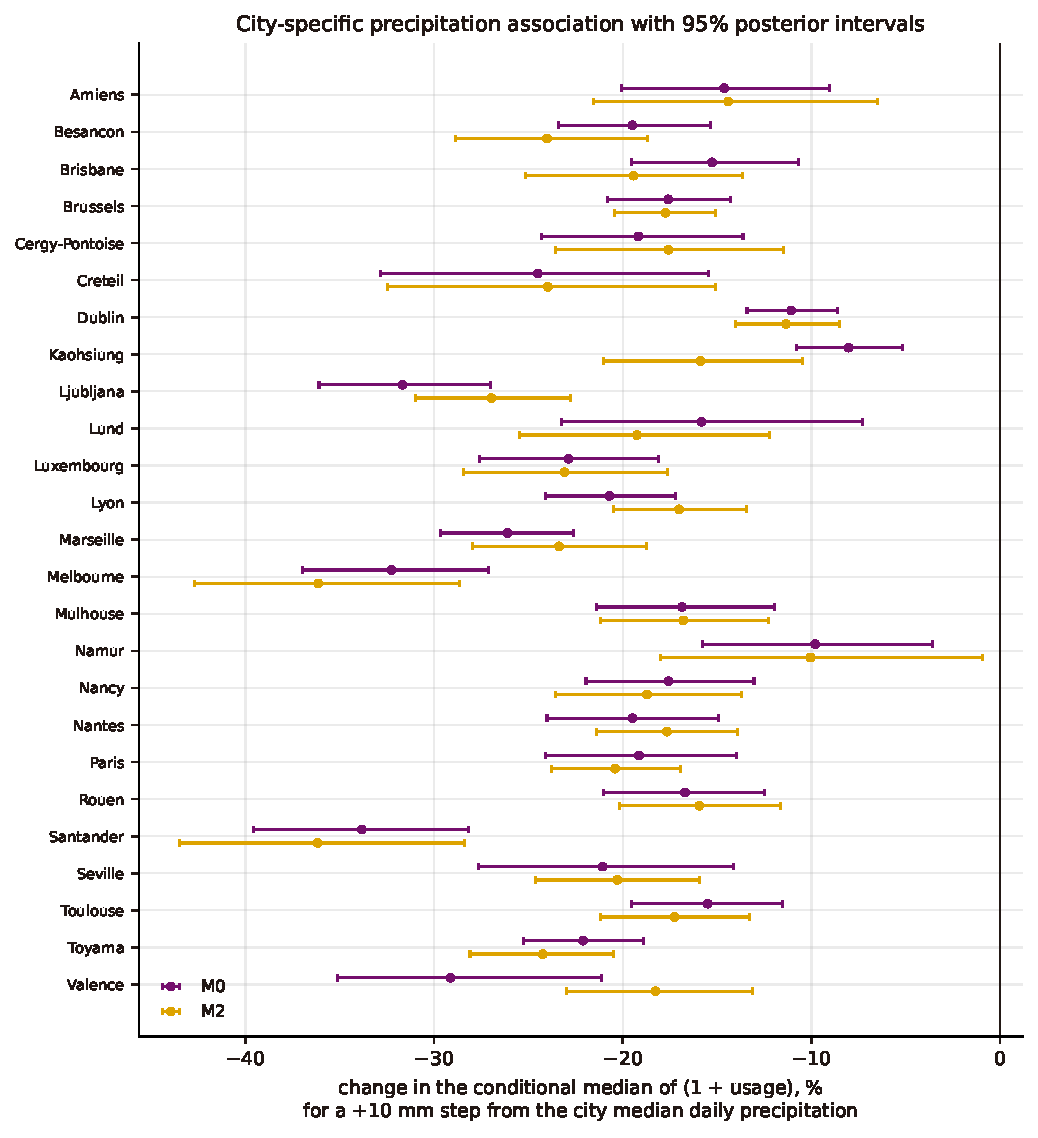
\includegraphics[width=\linewidth,height=5.25cm,keepaspectratio]{fig02_rain_forest.pdf}
    \end{column}
    \begin{column}{0.51\textwidth}
      \small
      \begin{alertblock}{Negative in every city}
        City-equal average:
        \par M2 \hl{\RainMTwoMed\%}, 95\% $[\RainMTwoLo,\RainMTwoHi]$.
        \par M0 \hl{\RainMZeroMed\%}, 95\% $[\RainMZeroLo,\RainMZeroHi]$.
      \end{alertblock}
      \footnotesize
      Contrast: $+10$ mm from city median daily precipitation.
      Percent change in the conditional median of $(1+\text{usage})$.
      \par\vspace{0.15cm}
      M2 city medians: \RainMTwoCityMin\% to \RainMTwoCityMax\%.
      Smallest $P(\beta_{\mathrm{rain}}<0)$: \RainMTwoMinPNeg.
      \par\vspace{0.15cm}
      Each specification uses its own saved fit. City ordering has not been tested pairwise.
    \end{column}
  \end{columns}
\end{frame}

% ---------------------------------------------------------------- 5（目标 35 秒）
\begin{frame}{Temperature: positive association, uncertain peak}
  \begin{columns}[c,onlytextwidth]
    \begin{column}{0.63\textwidth}
      \centering
      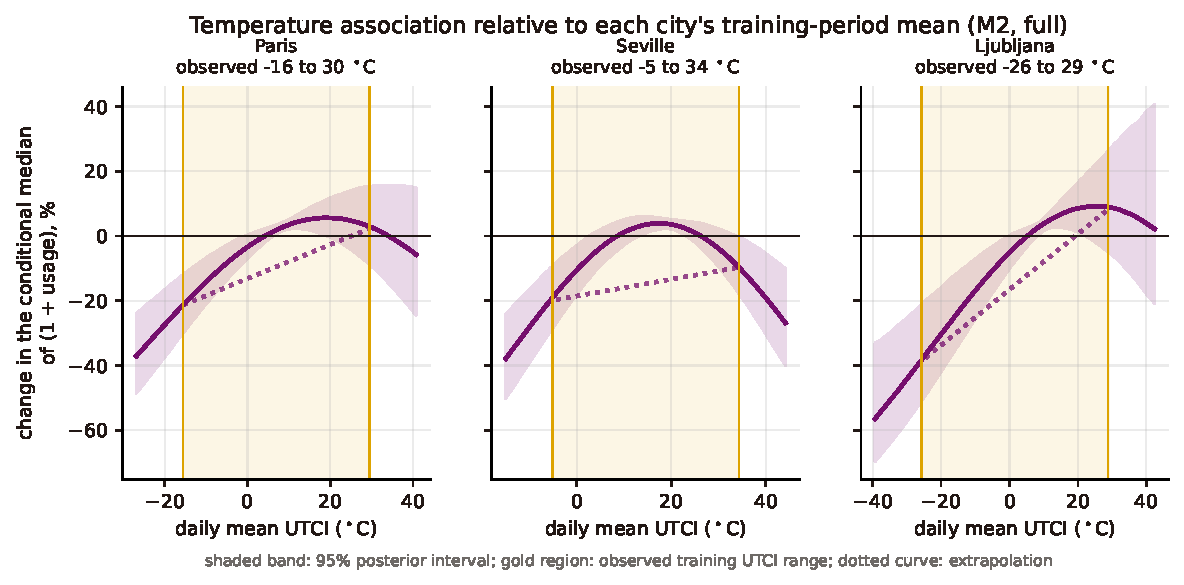
\includegraphics[width=\linewidth,height=4.60cm,keepaspectratio]{fig03_temperature_curves.pdf}
      \par\vspace{0.12cm}
      \footnotesize Curves: M2 full-period fit. M0/M2 contrasts use the same 25 cities and window.
      Peak location changes with the specification.
    \end{column}
    \begin{column}{0.33\textwidth}
      \footnotesize
      \begin{alertblock}{UTCI $+10^\circ$C}
        M0 \hl{\TempMZeroMed\%}
        \par 95\% $[\TempMZeroLo,\TempMZeroHi]$.
        \par\vspace{0.08cm}
        M2 \hl{\TempMTwoMed\%}
        \par 95\% $[\TempMTwoLo,\TempMTwoHi]$.
      \end{alertblock}
      Interior peak, $P>0.95$:
      \par M0 \PeakCitiesMZero{}/25; M2 \PeakCitiesMTwo{}/25.
      \par\vspace{0.12cm}
      $+10^\circ$C leaves the observed range in \ExtrapCitiesMTwo{} city: Kaohsiung.
      \par\vspace{0.12cm}
      Separate fits; no single optimal temperature is identified.
    \end{column}
  \end{columns}
\end{frame}

% ---------------------------------------------------------------- 6（目标 40 秒）
\begin{frame}{Sampling reliability and daily dependence}
  \begin{columns}[c,onlytextwidth]
    \begin{column}{0.60\textwidth}
      \centering
      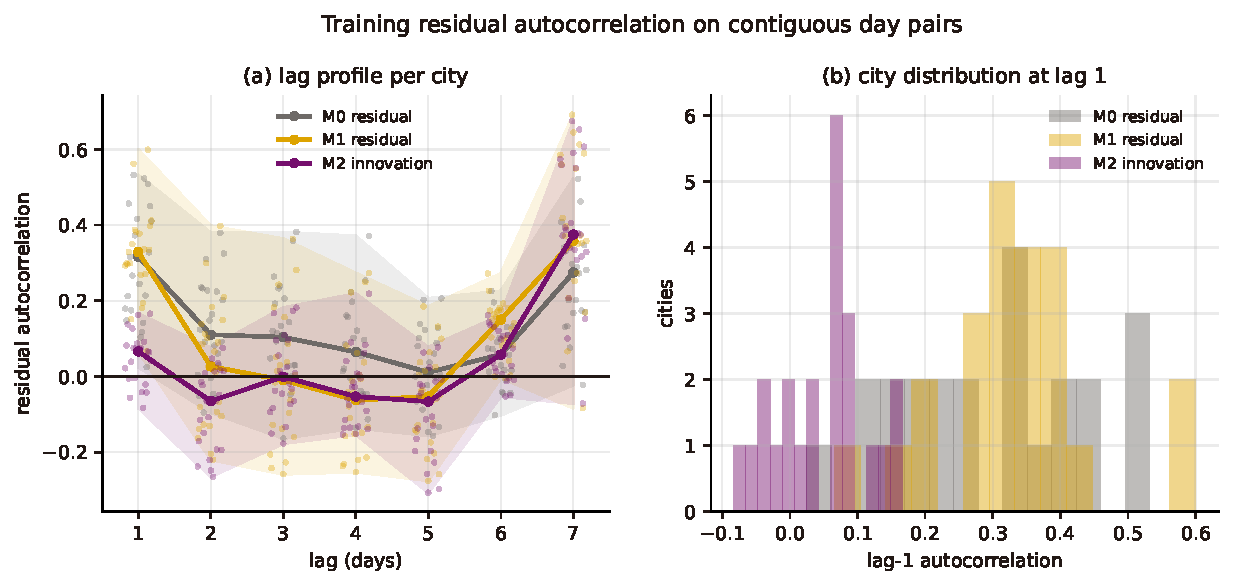
\includegraphics[width=\linewidth,height=4.25cm,keepaspectratio]{fig04_residual_acf.pdf}
      \par\vspace{0.12cm}
      \footnotesize M0/M1: fitted residuals. M2: innovations.
      \par Lower innovation correlation does not establish the contribution of AR(1) alone;
      the specifications change several structural components.
    \end{column}
    \begin{column}{0.36\textwidth}
      \footnotesize
      \begin{block}{All 11 core fits passed}
        \begin{tabular}{@{}lr@{}}
          Worst $\widehat{R}$ & \CoreMaxRhat \\
          Smallest bulk ESS & \CoreMinEss \\
          Smallest tail ESS & \CoreMinTailEss \\
          Divergences / depth hits & 0 / 0 \\
        \end{tabular}
      \end{block}
      Four chains, 3{,}000 warmup and 3{,}000 retained draws; seed 27.
      \par\vspace{0.12cm}
      \textbf{Dev 1: median lag-one}
      \par
        \begin{tabular}{@{}lr@{}}
          M0 fitted residual & \MZeroDevOneLagOne \\
          M1 fitted residual & \MOneDevOneLagOne \\
          M2 innovation & \MTwoDevOneLagOne \\
        \end{tabular}
      \par\vspace{0.12cm}
      Sampling, model fit and prediction require separate checks.
    \end{column}
  \end{columns}
\end{frame}

% ---------------------------------------------------------------- 7（目标 65 秒）
\begin{frame}{Prediction: gains vary across windows}
  \small
  \begin{columns}[T,onlytextwidth]
    \begin{column}{0.52\textwidth}
      \begin{block}{56-day block WIS \textperiodcentered\ lower is better}
        \begin{tabular}{@{}lrrr@{}}
          \toprule
          & dev 1 & dev 2 & final \\
          \midrule
          M0 & \MZeroDevOneWis & \MZeroDevTwoWis & \MZeroFinalWis \\
          M1 & \MOneDevOneWis & \MOneDevTwoWis & \MOneFinalWis \\
          M2 & \hl{\MTwoDevOneWis} & \hl{\MTwoDevTwoWis} & \MTwoFinalWis \\
          \bottomrule
        \end{tabular}
      \end{block}
      \footnotesize Paired seven-day block intervals, M2 minus M0:
      \par dev 1: $[\PairDevOneLo,\PairDevOneHi]$; includes zero.
      \par dev 2: $[\PairDevTwoLo,\PairDevTwoHi]$; excludes zero.
      \slidenote{The pre-specified development-fold rule selects M2.
      City-equal scores; one-step results in backup.}
    \end{column}
    \begin{column}{0.45\textwidth}
      \begin{alertblock}{Final-window calibration}
        \begin{tabular}{@{}lrr@{}}
          \toprule
          & M0 & M2 \\
          \midrule
          Block WIS & \MZeroFinalWis & \MTwoFinalWis \\
          90\% coverage & \MZeroFinalBlockCov\% & \MTwoFinalBlockCov\% \\
          \bottomrule
        \end{tabular}
      \end{alertblock}
      \footnotesize Wider M2 intervals and lower coverage indicate a mismatch between
      predictive distributions and observations.
      \slidenote{Final window previously inspected. No retuning after this evaluation.}
    \end{column}
  \end{columns}
\end{frame}

% ---------------------------------------------------------------- 8（目标 40 秒）
\begin{frame}{Findings and their scope}
  \small
  \begin{columns}[T,onlytextwidth]
    \begin{column}{0.31\textwidth}
      \begin{block}{01 \quad Precipitation}
        \hl{About \RainMTwoMed\%}
        \par per $+10$ mm; negative in every city.
        \par\vspace{0.14cm}
        \footnotesize Stable across two full-period specifications, two contrast definitions
        and three dev-1 model fits.
      \end{block}
    \end{column}
    \begin{column}{0.31\textwidth}
      \begin{block}{02 \quad Temperature}
        \hl{Positive full-period association}
        \par under both specifications.
        \par\vspace{0.14cm}
        \footnotesize Peak location changes with the specification.
        A single optimal temperature is not identified.
      \end{block}
    \end{column}
    \begin{column}{0.31\textwidth}
      \begin{block}{03 \quad Time structure}
        \hl{Development gains have limits}
        \par Final M2 coverage: \MTwoFinalBlockCov\%.
        \par\vspace{0.14cm}
        \footnotesize Lower innovation correlation and better development scores;
        final block worse than M0. AR(1)'s separate contribution is unverified.
      \end{block}
    \end{column}
  \end{columns}
  \slidenote{Observational associations; both prediction tasks condition on realised weather.
    Causal effects, climate adaptation and operational forecasting are outside the study scope.}
  \vspace{0.14cm}
  \centering \hl{Thank you \textperiodcentered\ Questions}
\end{frame}

% ================================================================ backup
\begin{frame}{Backup 1: priors and sampling}
  \footnotesize
  \begin{columns}[T,onlytextwidth]
    \begin{column}{0.50\textwidth}
      \begin{block}{Priors on the $\log(1+U)$ scale}
        \begin{tabular}{@{}ll@{}}
          Population intercept & $\mathcal{N}(7,2)$ \\
          City intercept scale & HN$(2)$ \\
          UTCI, per $10^\circ$C & $\mathcal{N}(0,0.5)$ \\
          Quadratic & $\mathcal{N}(0,0.3)$ \\
          Rainfall & $\mathcal{N}(0,0.3)$ \\
          Weekend & $\mathcal{N}(0,0.4)$ \\
          Weekday contrasts & $\mathcal{N}(0,0.4)$ \\
          Annual harmonic & $\mathcal{N}(0,0.8)$ \\
          Trend, per 100 days & $\mathcal{N}(0,0.3)$, HN$(0.3)$ \\
          AR persistence $z$ & $\mathcal{N}(0,0.5)$, HN$(0.5)$ \\
          Log noise scale & $\mathcal{N}(-0.5,0.8)$, HN$(0.5)$ \\
        \end{tabular}
      \end{block}
      \slidenote{HN denotes a half-normal distribution.}
    \end{column}
    \begin{column}{0.46\textwidth}
      Varying coefficients share the population-normal and half-normal group scale.
      Noise uses $0.8$ for the population and $0.5$ for the group.

      \vspace{0.10cm}
      Trend uses the fitted scale $0.3$. Configuration field
      \texttt{beta\_trend\_city\_sd}$=0.2$ is unused.

      \vspace{0.18cm}
      M2 dev 1 full prior predictive check, 1{,}000 draws: \PriorNegJoint\% below zero;
      intercept-only check: \PriorNegIntercept\%. The upper tail is wide.
      Source: \texttt{followup\_checks.json} in \texttt{logs/review/}.

      \vspace{0.18cm}
      Acceptance: $\widehat{R}\le1.01$, bulk and tail ESS $\ge400$, no divergences, MCSE below 5\%
      of the posterior standard deviation.
    \end{column}
  \end{columns}
\end{frame}

\begin{frame}{Backup 2: associations and prediction}
  \footnotesize
  \renewcommand{\arraystretch}{0.85}
  \begin{columns}[T,onlytextwidth]
    \begin{column}{0.55\textwidth}
      \centering
      \begin{tabular}{@{}lrr@{}}
        \toprule
        Contrast (\%) & M0 & M2 \\
        \midrule
        Rain $+10$ mm & $-19.98$ & $-20.21$ \\
        95\% interval & $[-21.07,-18.89]$ & $[-21.37,-18.99]$ \\
        Rain median--90th & $-16.40$ & $-16.99$ \\
        95\% interval & $[-17.28,-15.53]$ & $[-18.02,-15.95]$ \\
        UTCI $+10^\circ$C & $5.22$ & $6.16$ \\
        95\% interval & $[3.67,6.76]$ & $[4.12,8.32]$ \\
        UTCI 25th--75th & $19.89$ & $14.04$ \\
        95\% interval & $[17.44,22.47]$ & $[11.11,17.27]$ \\
        Interior peak & 15/25 & 5/25 \\
        Outside range & 1/25 & 1/25 \\
        \bottomrule
      \end{tabular}
      \par\vspace{0.04cm}
      City-equal percentages, 25 systems; 95\% intervals.
      Peak: $P>0.95$; outside range: UTCI $+10^\circ$C.
    \end{column}
    \begin{column}{0.43\textwidth}
      \centering
      \begin{tabular}{@{}lrr@{}}
        \toprule
        Method (MAE) & Block & One-step \\
        \midrule
        M0 & 0.3207 & 0.3207 \\
        Seasonal naive & 0.4252 & 0.3421 \\
        City AR-OLS & 0.5192 & 0.3197 \\
        City OLS & 0.5208 & 0.5208 \\
        M2 & 0.5547 & 0.3601 \\
        City constant & 0.5551 & 0.5551 \\
        \bottomrule
      \end{tabular}
      \par\vspace{0.04cm}
      Final city-equal MAE; lower is better. Naive: 7-day lag; OLS: parameter uncertainty.
      Baselines compare points only.
    \end{column}
  \end{columns}
  \vspace{0.04cm}
  Final one-step WIS: M0 \MZeroFinalStepWis{}, M2 \MTwoFinalStepWis{};
  90\% coverage: \MZeroFinalStepCov\% and \MTwoFinalStepCov\%, respectively.
  \par\vspace{0.04cm}
  Dev 1 temperature, 23 cities: M0
  \TempMZeroDevOneMed\% ($[\TempMZeroDevOneLo,\TempMZeroDevOneHi]$), M1 \TempMOneDevOneMed\%, M2
  \TempMTwoDevOneMed\% ($[\TempMTwoDevOneLo,\TempMTwoDevOneHi]$).
  This window and roster differ from the full-period fits.
\end{frame}

\begin{frame}{Backup 3: limitations and reproduction}
  \footnotesize
  \setbeamerfont{itemize/enumerate body}{size=\footnotesize}
  \begin{columns}[T,onlytextwidth]
    \begin{column}{0.50\textwidth}
      \begin{block}{Limitations}
        \begin{itemize}
          \setlength{\itemsep}{0.06cm}
          \item Student-$t$ permits negative log usage. Expected usage does not exist for finite
            $\nu$; report medians and quantiles.
          \item M0 leaves lag-one residual autocorrelation near \MZeroDevOneLagOne.
          \item Sampling, model fit and prediction require separate checks.
          \item Both tasks condition on realised weather.
          \item The final block was inspected before this analysis.
        \end{itemize}
      \end{block}
    \end{column}
    \begin{column}{0.48\textwidth}
      \begin{block}{Files}
        \begin{itemize}
          \setlength{\itemsep}{0.06cm}
          \item Data: Mendeley Data, Version 1, CC BY 4.0.
            Cleaned CSV in \texttt{data/}; SHA-256 checked before fitting.
          \item Bean, Pojani and Corcoran (2021), \emph{Journal of Transport Geography}, 95:103155.
          \item PyMC 6.3.2, nutpie 0.16.11; NUTS, four chains.
          \item Commands: \texttt{src/run.py}. Tests in \texttt{tests/};
            verification: \texttt{src/verify\_deliverables.py}.
        \end{itemize}
      \end{block}
    \end{column}
  \end{columns}
\end{frame}

\end{document}
